\documentclass[a4paper,12pt]{article}

\usepackage{abakos}
\usepackage{abntex2cite} 

%%%%%%%%%%%%%%%%%%%%%%%%%%%
%Capa da revista
%%%%%%%%%%%%%%%%%%%%%%%%%%

\setLogoRevista{figuras/logo-revista.png}
\setCheckForUpdatesUrl{http://link.com}

\newcommand{\secaoNome}{Seção do Artigo}
\newcommand{\editorNome}{Nome completo}

% Datas do artigo
\newcommand{\dataRecebido}{31/03/2025}
\newcommand{\dataAprovado}{28/05/2025}
\newcommand{\dataPublicado}{05/06/2025}

% PID e DOI
\newcommand{\pidArtigo}{10.0000/0000-0000-idartigo}
\newcommand{\doiArtigo}{https://doi.org/10.0000/0000-0000-idartigo}

% Tipo da licença:
\tipoLicenca{CC-BY}
%\tipoLicenca{CC-BY-SA}
%\tipoLicenca{CC-BY-NC}
%\tipoLicenca{CC-BY-ND}
%\tipoLicenca{CC-BY-NC-SA}
%\tipoLicenca{CC-BY-NC-ND}

% Blocos textuais
\newcommand{\textoLicenca}{Texto padrão da licença\par Texto texto texto texto texto texto texto.}
\newcommand{\textoCopyright}{Texto texto texto texto texto texto texto texto texto texto.}
\newcommand{\textoCRediT}{Texto texto texto texto texto texto texto texto texto texto.}
\newcommand{\textoConflito}{Texto texto texto texto texto texto texto texto texto texto.}
\newcommand{\textoFinanciamento}{Texto texto texto texto texto texto texto texto texto texto.}

\newcommand{\editorial}{\textbf{Nome da Revista}, Cidade, v. 1, n. 1, p. 00-00, Jul. 2025 - ISSN: 0000-0000 DOI: 00.00000/xxxxxxxx}  

%%%%%%%%%%%%%%%%%INFORMAÇÕES SOBRE AUTORES %%%%%%%%%%%%%%%%%%%%%%%%%%%%%%%

%%%%%%
%%Lembre-se de submeter a versão não identificada!
%%%%%%

% Define afiliações
\afiliacao{1}{Instituto X, Departamento Y, Universidade Z}
\afiliacao{2}{Laboratório ABC, Universidade DEF}

% Define autores
\autor{João}{da Silva}{1}{https://orcid.org/0000-0000-0000-0001}
\autor{Lucas}{Costa}{2}{https://orcid.org/0000-0000-0000-0002}
\autor{José}{Souza}{1}{https://orcid.org/0000-0000-0000-0003}

% E-mail de contato
\emailCorrespondencia{email\_responsavel@mail.com}


% ======= PORTUGUÊS =======
\newcommand{\monog}{Título do Artigo em Português}

\newcommand{\resumoPT}{
	\noindent\textbf{Resumo:} Por favor, forneça um resumo com no máximo 250 palavras. Seu resumo deve explicar as principais contribuições do seu artigo e não deve conter nenhum material que não esteja incluído no texto principal.
}

\newcommand{\keywordsPT}{termo1; termo2; termo3; termo4; termo5.}

% ======= INGLÊS =======
\newcommand{\monogIngles}{Título do artigo em Inglês}

\newcommand{\resumoEN}{
	\noindent\textbf{Abstract:} Please provide an abstract with a maximum of 250 words. It should explain the main contributions of your article and must not contain any material not included in the main text.
}

\newcommand{\keywordsEN}{term1; term2; term3; term4; term5.}

% ======= ESPANHOL =======
\newcommand{\monogEspanhol}{Título do artigo em Espanhol}

\newcommand{\resumoES}{
	\noindent\textbf{Resumen:} Por favor, proporcione un resumen de un máximo de 250 palabras. Debe explicar las principales contribuciones de su artículo y no debe contener ningún material que no esté incluido en el texto principal.
}

\newcommand{\keywordsES}{término1; término2; término3; término4; término5.}

% Como citar
\newcommand{\comoCitar}{%
	\textit{Nome da Revista}, Cidade, v. 23, p. x--xx, 2025. DOI: https://doi.org/10.0000/0000-0000-0000.
}

\begin{document}

% %%%%%%%%%%%%%%%%%%%%%%%%%%%%%%%%%%
% %% Pagina de titulo
% %%%%%%%%%%%%%%%%%%%%%%%%%%%%%%%%%%

\revistaheader
\newpage

\selectlanguage{brazilian}
 \onehalfspace  % espaçamento 1.5 entre linhas
 \setlength{\parindent}{1.25cm}

%%%%%%%%%%%%%%%%%%%%%%%%%%%%%%%%%%%%%%%%%%%%%%%%%
%% INICIO DO TEXTO
%%%%%%%%%%%%%%%%%%%%%%%%%%%%%%%%%%%%%%%%%%%%%%%%%

\section{Introdução}

Este documento apresenta o modelo dos manuscritos a serem submetidos e possivelmente publicados na revista Abakós. Este template\footnote{Todas as palavras em língua estrangeira devem vir em itálico, com exceção do abstract e títulos de obras na lista de referência} segue o formato desejado. Portanto, os autores podem editar este documento incluindo o conteúdo do seu trabalho científico, tomando o cuidado de preservar a formatação.
De forma geral, todo o texto de desenvolvimento do artigo, da introdução às considerações finais, deve estar de acordo com as seguintes diretrizes:
\begin{itemize}
    \item Parágrafos recuados a 1,25 centímetros;
    \item Texto com tamanho 12;
    \item Fonte Times New Roman;
    \item Espaçamento entre linhas de 1,5;
    \item Texto em formato justificado.
\end{itemize}

No restante deste documento, a Seção~\ref{sec:sec} apresenta as diretrizes para a formatação de seções e subseções. A Seção~\ref{sec:figTabEqAlg}, por sua vez, apresenta as diretrizes para a inclusão de figuras, tabelas, equações e algoritmos como parte do texto do artigo. Em seguida, a Seção~\ref{sec:ref} apresenta as diretrizes sobre o formato da lista de referências e da citação de artigos como parte do texto. Por fim, a Seção~\ref{sec:con} apresenta diretrizes sobre a seção de conclusão do trabalho.


\section{Formatação de Seções e Subseções}
\label{sec:sec}

Em todo o texto, os títulos das seções devem utilizar a formatação caixa alta, negrito, tamanho 12. Todo título de seção ou subseção deverá ser seguido de texto. Para as seções textuais utilizar numeração progressiva em algarismos arábicos, limitada até a seção quinária. Devem ser diferenciadas utilizando os recursos gráficos \cite{manualpucartigo}.

Os títulos das subseções secundárias são formatados em caixa baixa, negrito, tamanho 12. Os títulos das subseções terciárias são formatados em caixa baixa, itálico, negrito, tamanho 12. Por fim, os títulos das subseções quaternária são formatados em caixa baixa, sublinhado, negrito, tamanho 12. Como exemplo, seguem as subseções apresentadas nesta seção com títulos no formato desejado.

\subsection{Exemplo de Subseção Secundária}
\subsubsection{Exemplo de Subseção Terciária}
\subsubsubsection{Exemplo de Subseção Quaternária}


\section{Figuras, Tabelas, Equações e Algoritmos}
\label{sec:figTabEqAlg}

Imagens, tabelas, algoritmos devem ser incluídos de forma centralizada, dentro das margens. Para gráficos, quadros e tabelas, cujos dados foram extraídos da própria pesquisa, deve-se  usar a expressão “Dados da pesquisa” ao indicar a fonte.

\subsection{Figuras}

Telas de \textit{software}, mapas, gráficos e diagramas devem ser inseridas como figuras, indicando a fonte e referenciadas no texto. A Figura \ref{fig:figura1} apresenta o processo de revisão de trabalhos submetidos à revista Abakós, como um exemplo de figura que contém diagrama. Observe que, no caso dessa figura, a fonte é indicada como ``Dados da Pesquisa'', indicando que a figura não foi obtida de terceiros, mas elaborada pelos próprios autores, no caso, os editores da revista.

% Figura
\begin{figure}[htb]
	\centering	
	\caption[Processo de Revisão da Revista Abakós.]{Processo de revisão da revista Abakós}
	\label{fig:figura1}
	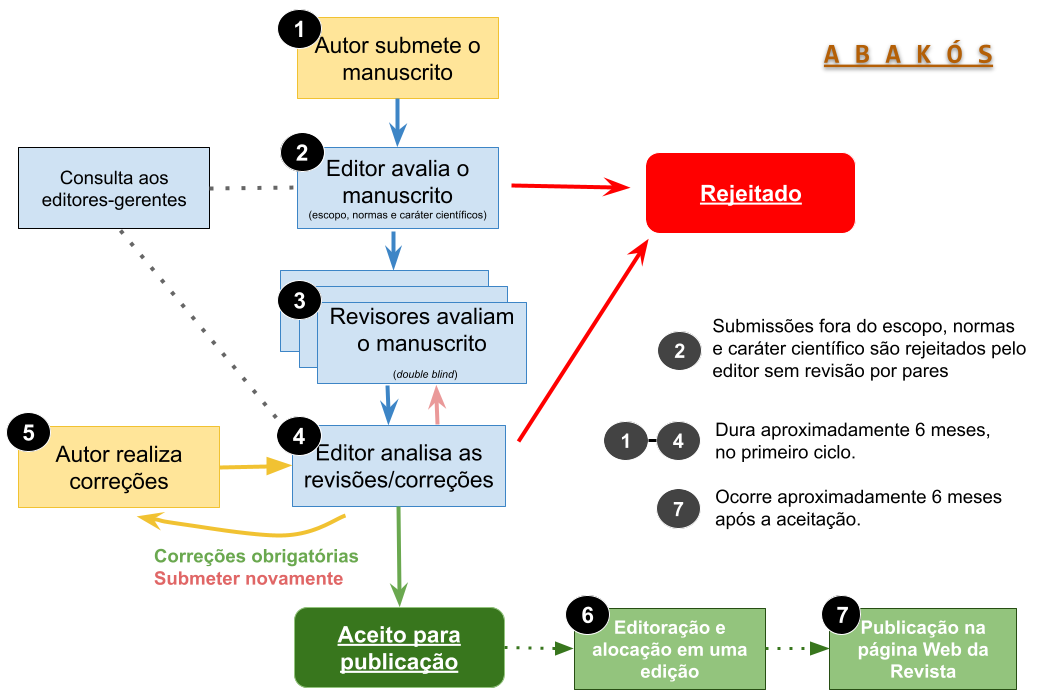
\includegraphics[width=0.8\textwidth]{figuras/Abakos-review.png}\\
	\textbf{\footnotesize Fonte: Dados da Pesquisa.}
\end{figure}

A Figura~\ref{fig:figura2}, por sua vez, é um mapa que destaca a localização do Instituto de Ciências Exatas (ICEI) no campus da PUC Minas no Coração Eucarístico, na cidade de Belo Horizonte, estado de Minas Gerais, Brasil. Observe que, no caso dessa figura, a fonte é indicada como “{\it Google Maps}	\footnote{Disponível em: \url{https://www.google.com.br/maps}.Acessado em: 12 de abr. de 2021.}”, que é um sistema de pesquisa e visualização de mapas e imagens de satélite. Encontram-se indicados também o endereço eletrônico de tal sistema e a data em que a captura foi feita. Sempre atentar para os direitos autorais das figuras de terceiros utilizadas no artigo, isto é responsabilidade dos autores.

\begin{figure}[ht]
	\centering	
	\caption[Mapa com a localização do ICEI.]{Mapa com a localização do ICEI no campus da PUC Minas}
	\label{fig:figura2}
	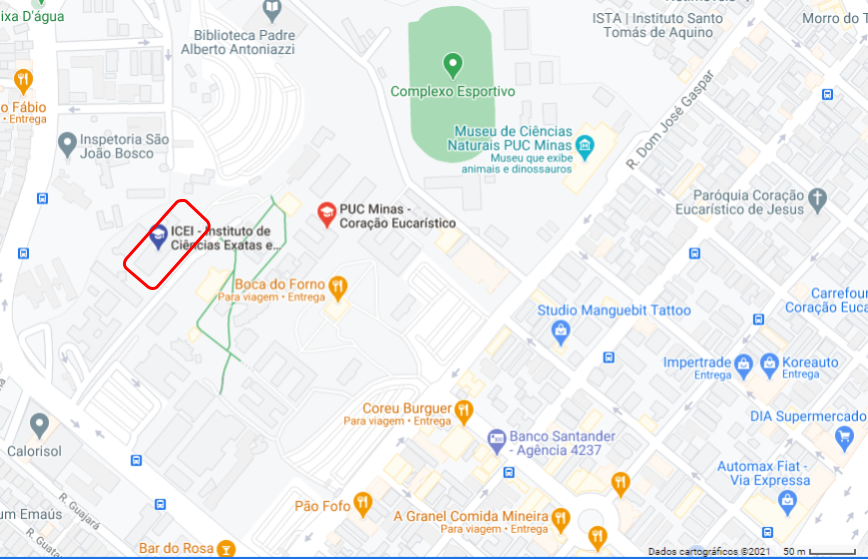
\includegraphics[width=0.6\textwidth]{figuras/Mapa-ICEI-PUCMinas.png}\\
	\textbf{\footnotesize Fonte: Google Maps.}
\end{figure}

A Figura~\ref{fig:figura3} é um exemplo de como inserir um gráfico no corpo do texto. É importante observar que o gráfico segue o mesmo padrão das outras figuras. Cada figura inserida precisa ser citada e contextualizada no texto. Por exemplo, a Figura~\ref{fig:figura3} mostra que, para o período entre os anos de 2014 a 2020, o número médio anual de autores por artigo publicado na revista Abakós foi de aproximadamente três autores por artigo, com maior oscilação nos anos de 2014 a 2016.

\begin{figure}[ht]
	\centering	
	\caption[Média de Autores por Artigo.]{Número médio de autores em artigos publicados na revista Abakós por ano, do ano de 2014 ao ano de 2020}
	\label{fig:figura3}
	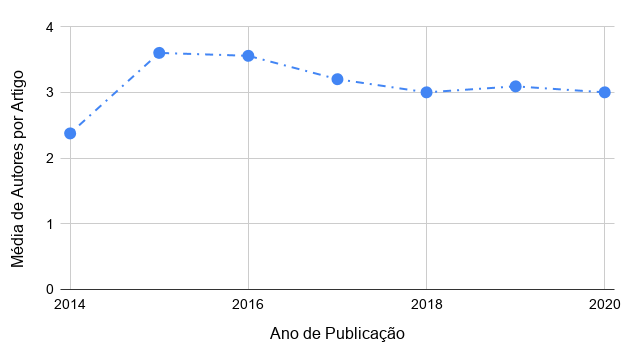
\includegraphics[width=0.8\textwidth]{figuras/AutoresPorArtigoNaRevistaAbakos.png}\\
	\textbf{\footnotesize Fonte: Dados da Pesquisa.}
\end{figure}



\subsection{Tabelas}

Informações tabuladas em linhas e colunas devem ser apresentadas no texto como tabelas, de modo a facilitar a análise dos dados. Por exemplo, tabelas que apresentam dados estatísticos devem ser abertas nas laterais, com espaços verticais separando as colunas e sem espaços horizontais, exceto na separação do cabeçalho. Dados textuais esquemáticos, comparativos ou descritivos que estejam apresentados em formato de linhas e colunas também devem ser incluídos no texto como tabelas. A Tabela \ref{tab:tabela1} apresenta a quantidade de artigos e edições publicadas pela revista Abakós por ano entre 2016 e 2020, como um exemplo de tabela.

% Tabela
\begin{table}[ht]
	\centering
	\caption{Número de artigos e edições publicados pela revista Abakós entre 2016 e 2020}
	\label{tab:tabela1}
	% Conteúdo da tabela
	\begin{tabular}{l|c|c}
  \hline
    \textbf{Ano}	& \textbf{Número de artigos} & \textbf{Número de edições} \\
    \hline
     2020	& 11 &  2 \\
     2019	& 12 &  2 \\
     2018	& 10 &  2 \\
     2017   & 10  &  2 \\
     2016	& 10  &  2 \\
     \hline
 \end{tabular}
	{\footnotesize\\ \textbf{Fonte: Dados da Pesquisa.}}
\end{table}


\subsection{\esp Equações}

As equações podem ser apresentadas dentro do texto, usando o formato matemático. Esse é o caso de descrever $y=x^2+1$, pois é parte da frase e está dentro do parágrafo. Idealmente, equações mais complexas devem ser apresentadas fora do fluxo do texto e referenciadas no texto pelos seus números. Esse é o caso da Equação~\ref{eq:aid}, da Equação~\ref{eq:bid} e da Equação~\ref{eq:qscore}, que foram propostas na literatura como formas de calcular a credibilidade de seres humanos ao realizarem computação em seus sistemas cognitivos~\cite{ponciano2018agreement}. 

\begin{equation}
\label{eq:aid}
y_{i,d}=\frac{\displaystyle\sum_{w\in Y_{i,d}}s_{w,d}}{|Y_{i,d}|}
\end{equation}

\begin{equation}
\label{eq:bid}
x_{i,d}=\frac{\displaystyle\sum_{w\in X_{i,d}}s_{w,d}}{|X_{i,d}|}
\end{equation}

\begin{equation}
\label{eq:qscore}
r_{i,d} = \frac{s_{i,d} + y_{i,d}-x_{i,d} + 1}{3}, r_{i,d}\in[0,1]
\end{equation}

\subsection{Algoritmos}

Algoritmos podem ser inseridos no texto texto e referenciados pelo seu número. Esse é o caso do Algoritmo~\ref{alg:max}. O algoritmo deve explicitar as entradas (\textit{inputs}) e saídas (\textit{outputs}). No caso do Algoritmo~\ref{alg:max}, a entrada é um vetor de números ($list$) e a saída é o maior valor no vetor (definido como $biggest\_item$). Cada linha dos passos de computação do algoritmo deve ser numerada. O pacote \LaTeX~ recomendado é o \textit{algorithmic}, que é usado nesse exemplo.

\begin{algorithm}
\caption{Valor Máximo no Vetor}
\label{alg:max}
\begin{algorithmic}[1]
\REQUIRE $list$
\ENSURE $biggest\_item$
    \STATE $biggest\_item \Leftarrow list[0]$
    \FORALL{$item$ in $list$}
        \IF{$item > biggest\_item$}
            \STATE $biggest\_item \Leftarrow item$
        \ENDIF
    \ENDFOR
\end{algorithmic}
\end{algorithm}

\section{Dicas: Citações e Referências}
\label{sec:ref}

Tanto as citações como as referências citadas no texto devem seguir as normas da ABNT, recomenda-se fortemente consultar o documento de Elaboração de Referências~\cite{manualpucref} \footnote{Disponível em: \url{http://portal.pucminas.br/biblioteca/documentos/Guia-ABNT-referencias.pdf}. Acesso em: 06 de Mai. de 2021.} e ao documento de citações e referências~\cite{manualpuccit}\footnote{Disponível em: \url{http://portal.pucminas.br/biblioteca/documentos/citacoes-referencias.pdf}. Acesso em: 06 de Mai. de 2021.}.

\subsection{Como fazer citações no texto}

Para citar trabalhos científicos (artigo, livro, etc) no texto, deve-se trazer o sobrenome do autor/autores e a data da publicação, como nos exemplos abaixo:

\begin{itemize}
    \item ``De acordo com Dickman e Ponciano (2020)...'' \textit{[Em letras minúsculas caso venha no texto]}
    \item ``Os dados divergiram como previsto em trabalhos da literatura (DICKMAN; PONCIANO, 2020)'' \textit{[Em caixa alta caso venha em parênteses]}
    \item Para três autores ou mais deve-se usar ``Dickman et al. (2020)'', no texto ou "(DICKMAN et al., 2020)".
\end{itemize}

Todas as referências citadas no texto devem ser listadas no final do trabalho. Observe que trabalhos que não foram citados NÃO devem ser relacionados na lista final.

\subsection{Como elaborar a lista de referências}

As referências devem ser organizadas em ordem alfabética de acordo com o último sobrenome do primeiro autor. Caso haja mais de uma obra do mesmo autor, a ordem deve obedecer a ordem de chamada no texto.

É importante observar que uniformizamos as citações de modo que apenas as iniciais dos nomes devem ser utilizadas, como em: DICKMAN, A. G.; PONCIANO, L. 

A seguir mostramos como montar a lista de referências, para maiores detalhes consultar os {\it links} disponibilizados acima:

\begin{itemize}
    \item Para livro~\cite{arroyo}: \\

\noindent ARROYO, M. G. {\bf Ofício de mestre}: Imagens e auto-imagens. 15.ed. Petrópolis: Vozes, 2013.

    \item Para capítulo de livro~\cite{bordieu}: \\

\noindent BORDIEU, P. Espaço social e espaço simbólico. {\it In}: BORDIEU, P. {\bf Razões práticas}: sobre a teoria da ação. 11.ed. Tradução: Mariza Corrêa. Campinas: Papirus, 2011. cap.1, pp.13.27.

    \item Para artigo em periódico~\cite{ferreira}: \\
    
\noindent FERREIRA, A.C.; DICKMAN, A.G. História oral: um método para investigar o ensino de física para estudantes cegos. {\bf Revista Brasileira de Educação Especial}, v.21, n.2, p.245-58, 2015.

    \item Para trabalho em atas/anais de eventos~\cite{kogut}:
    
\noindent KOGUT, M.C. A formação docente: Os saberes e a identidade do professor. {\it In}: CONGRESSO NACIONAL DE EDUCAÇÃO, 12., 2015, Curitiba. Anais {\bf […]}. Curitiba: PUCPR, 2015.

\item Para dissertação~\cite{exemplodiss}:
\noindent PERTENCE, M.L.B. {\bf Ensino de física para estudantes cegos}: Oficina sobre criação e adaptação de materiais didáticos para professores e licenciandos. 2021. Dissertação (Mestrado em Ensino) - Pontifícia Universidade Católica de Minas Gerais, Belo Horizonte, 2021.

\item Para tese~\cite{exemplotese}:
\noindent DICKMAN, A.G. {\bf Transições de Fases de Não-equilíbrio em Sistemas de Partículas Interagentes} 1996. Tese (Doutorado em Física) - Universidade Federal de Minas Gerais, Belo Horizonte, 1996.
\end{itemize}

Na lista de referências, estão incluídos exemplos de artigos em anais de eventos~\cite{ponciano2017designing}, artigos em periódicos~\cite{ponciano2018agreement}, livro~\cite{swokowski1994} e capítulo de livros.

\section{Considerações Finais}
\label{sec:con}

A seção de Considerações Finais (ou Conclusão) deve estar de acordo com os objetivos do trabalho. Ela não deve apresentar novos resultados, citações ou interpretações de outros autores. Uma conclusão pode ser estruturada em partes. A primeira parte é um sumário do trabalho, relembrando o problema, objetivos e abordagem metodológica empregada. A segunda parte é uma descrição dos principais resultados e contribuições que se encontram reportados no trabalho. É importante relacionar os resultados obtidos com aqueles encontrados na literatura, discutidos no referencial teórico do trabalho. Por fim, a terceira parte é uma discussão de trabalhos relacionados que se mostram promissores a partir dos resultados obtidos.


%%%%%%%%%%%%%%%%%%%%%%%%%%%%%%%%%%%
%% FIM DO TEXTO
%%%%%%%%%%%%%%%%%%%%%%%%%%%%%%%%%%%

%%%%%%%%%%%%%%%%%%%%%%%%%%%%%%%%%%%
%% Inicio bibliografia
%%%%%%%%%%%%%%%%%%%%%%%%%%%%%%%%%%%

\newpage

\bibliographystyle{abntex2-alf}
\bibliography{bibliografia}

\end{document}